\documentclass[letterpaper]{article}
\usepackage[margin=1in]{geometry}
\usepackage[utf8]{inputenc}
\usepackage{textcomp}
\usepackage{amssymb}
\usepackage{natbib}
\usepackage{graphicx}
\usepackage{gensymb}
\usepackage{amsthm, amsmath, mathtools}
\usepackage[dvipsnames]{xcolor}
\usepackage{enumerate}
\usepackage{mdframed}
\usepackage[most]{tcolorbox}
\usepackage{csquotes}
% https://tex.stackexchange.com/questions/13506/how-to-continue-the-framed-text-box-on-multiple-pages

\tcbuselibrary{theorems}

\newcommand{\R}{\mathbb{R}}
\newcommand{\Z}{\mathbb{Z}}
\newcommand{\N}{\mathbb{N}}
\newcommand{\Q}{\mathbb{Q}}
\newcommand{\C}{\mathbb{C}}
\newcommand{\code}[1]{\texttt{#1}}
\newcommand{\mdiamond}{$\diamondsuit$}
\newcommand{\PowerSet}{\mathcal{P}}
\newcommand{\Mod}[1]{\ (\mathrm{mod}\ #1)}
\DeclareMathOperator{\lcm}{lcm}

%\newtheorem*{theorem}{Theorem}
%\newtheorem*{definition}{Definition}
%\newtheorem*{corollary}{Corollary}
%\newtheorem*{lemma}{Lemma}
\newtheorem*{proposition}{Proposition}


\newtcbtheorem[number within=section]{theorem}{Theorem}
{colback=green!5,colframe=green!35!black,fonttitle=\bfseries}{th}

\newtcbtheorem[number within=section]{definition}{Definition}
{colback=blue!5,colframe=blue!35!black,fonttitle=\bfseries}{def}

\newtcbtheorem[number within=section]{corollary}{Corollary}
{colback=yellow!5,colframe=yellow!35!black,fonttitle=\bfseries}{cor}

\newtcbtheorem[number within=section]{lemma}{Lemma}
{colback=red!5,colframe=red!35!black,fonttitle=\bfseries}{lem}

\newtcbtheorem[number within=section]{example}{Example}
{colback=white!5,colframe=white!35!black,fonttitle=\bfseries}{def}

\newtcbtheorem[number within=section]{note}{Important Note}{
        enhanced,
        sharp corners,
        attach boxed title to top left={
            xshift=-1mm,
            yshift=-5mm,
            yshifttext=-1mm
        },
        top=1.5em,
        colback=white,
        colframe=black,
        fonttitle=\bfseries,
        boxed title style={
            sharp corners,
            size=small,
            colback=red!75!black,
            colframe=red!75!black,
        } 
    }{impnote}
\usepackage[utf8]{inputenc}
\usepackage[english]{babel}
\usepackage{fancyhdr}
\usepackage[hidelinks]{hyperref}

\pagestyle{fancy}
\fancyhf{}
\rhead{CSE 131}
\chead{Friday, May 19, 2023}
\lhead{Lecture 21}
\rfoot{\thepage}

\setlength{\parindent}{0pt}

\begin{document}

\section{Optimization (Continued)}
This section continues the previous section.

\subsection{Optimization: Register Allocation}
Let's consider the following code: 
\begin{verbatim}
    (let (n (+ 5 9))
        (let (m (+ 2 3))
            (let (x (+ n 1))
                (let (y (+ m 2))
                    (+ x y)))))\end{verbatim}

The corresponding assembly\footnote{With tag checks removed to make the assembly more concise.}, along with the corresponding code from the above, is shown below.
\begin{verbatim}
    sub rsp, 40
      mov rax, 10
      mov [rsp + 0], rax    ; LHS of (+ 5 9)
      mov rax, 18
      add rax, [rsp + 0]

      mov [rsp + 0], rax    ; Variable n in (let (n ...))

      mov rax, 4
      mov [rsp + 8], rax    ; LHS of (+ 2 3)
      mov rax, 6
      add rax, [rsp + 8]

      mov [rsp + 8], rax    ; Variable m

      mov rax, [rsp + 0]    ; Variable n lookup 
      mov [rsp + 16], rax   ; LHS of (+ n 1)
      mov rax, 2
      add rax, [rsp + 16]

      mov [rsp + 16], rax   ; Variable x

      mov rax, [rsp + 8]    ; Variable m lookup 
      mov [rsp + 24], rax   ; LHS of (+ m 2)
      mov rax, 4
      add rax, [rsp + 24]

      mov [rsp + 24], rax   ; Variable y 

      mov rax, [rsp + 16]   ; Variable x lookup 
      mov [rsp + 32], rax
      mov rax, [rsp + 24]   ; Variable y lookup 
      add rax, [rsp + 32]
    add rsp, 40\end{verbatim}
One thing to notice immediately is that we reused some memory locations. One example is \code{[rsp + 8]}, which is where we stored both a temporary for addition and a value associated with a variable. We can generalize how many memory locations we ultimately \emph{will} use by using the \code{depth} function. In particular, if $\code{depth(expr)} \leq \text{Available Registers}$, then we can avoid memory entirely.

\bigskip 

There are two questions we should now consider.
\begin{enumerate}
    \item (\code{x86\_64}.) What registers should we use?
    \begin{mdframed}
        We can use the registers \code{rbx}, \code{r12}, \code{r13}, \code{r14}, which are callee-saved registers. Note that we aren't using \code{r15} because this register is specifically the heap pointer.
    \end{mdframed}
    \item (Design.) How should we implement this?
    \begin{mdframed}
        We can create a \code{Loc} \emph{enum} that holds either a register or a stack location (offset). Then, our environment can be represented by \code{HashMap<String, Loc>}.

        \bigskip 

        Suppose we have a list of registers that we can use. We can create a \code{get\_loc} function which takes a stack index and returns the new location to be used; this might look something like 
        \begin{verbatim}
    let regs = [...];
    get_loc(si):
        if si < regs.size():
            return regs[si];
        else:
            return Stack(si - regs.len());\end{verbatim}
        Then, we can use this location to update the environment, like 
        \begin{verbatim}
    ... 
    | ELet(x, val, body) => {
        env.update(x, get_loc(si));
    }\end{verbatim}
        Note that, while this is an \emph{improvement} to how our program is compiled, this can still be made a \emph{lot better}. Some other implementation notes to consider include: 
        \begin{itemize}
            \item We need to add code to save and restore registers in function definitions.
            \item We need to compute stack size based on \code{depth - available registers}.
        \end{itemize}
        Some improvements we could make to what we have so far include 
        \begin{itemize}
            \item Registers for outer bindings and stack for inner bindings. 
            \item Frequency matters. 
            \item Precompute registers and locations for all variables and temporaries across functions. 
            \item Are we using the minimal number of locations? (e.g., is the depth minimal?)
        \end{itemize}
    \end{mdframed} 
\end{enumerate}
\textbf{Remark:} The register allocation algorithm we're talking about, which uses an idea similar to \code{depth}, is similar to the \emph{Sethi-Ullman algorithm}.

\subsubsection{The Minimal Number of Locations}
Consider the following program: 
\begin{verbatim}
    (let (b 4)
        (let (x 10)
            (let (i (if input 
                        (let (z 11) (+ z b))
                        (let (y 9) (+ y 1))))
                (let (a (+ i 5))
                    (+ a x)))))\end{verbatim}
How many memory locations are needed? We'll look at the program from the \emph{end} to the beginning.
\begin{itemize}
    \item We first begin by looking at what variables are in use at the end. In this case, \code{a} and \code{x} are in use. The set of all variables in use is \[\{a, x\}.\]
    \item We're going to go back ``up'' the program. When we get to a \code{let}-bindings, we're going to remove it from the set of variables that are in use right now. In the next level, we're \emph{using} \code{i} and \code{x}, but we aren't using \code{a} here since \code{a} is being created. The set of all variables in use is \[\{i, x\}.\]
    \item The \code{if}-expression is more interesting. We need to consider both branches of the \code{if}-expression and do some unioning with the set of all variables in use. 
    \begin{itemize}
        \item Looking at the end of the ``else'' branch, at the body of the \code{let} binding, notice how \code{y} is being used. \code{x} and \code{i} are still around. The set of all variables in use is \[\{y, i, x\}.\]
        \item Looking at the end of the ``then'' branch, at the body of the \code{let} binding, notice how \code{z} and \code{b}\footnote{Even though \code{b} is defined at the top, this is the first time we're seeing \code{b} in use.} are in use. As usual, \code{x} and \code{i} are still around. The set of all variables in use is \[\{z, b, i, x\}.\]
        \item Here, we need to union the two branches. So, this gives us the variables in use
        \[\{z, b, i, x, y\}.\]
    \end{itemize}
    \item At the \code{let}-binding for \code{i} (\emph{not} in the body), we no longer have \code{z} or \code{y}, and \code{i} is being initialized here (so we aren't using \code{i} here). Thus, this gives us the variables in use \[\{x, b\}.\] 
    \item Moving ``up'' the program to the \code{let}-binding for \code{x}, we now only have the variables in use $\{x\}$. 
    \item Finally, moving ``up'' the program to the \code{let}-binding for \code{b}, we have the variables in use $\emptyset$. 
\end{itemize}
This information is telling us what variables need to be stored at the same time. Something we can do with this information is turn this into a \textbf{graph} where there's an edge between two variables \emph{if} they're in use at the same time. 
\begin{center}
    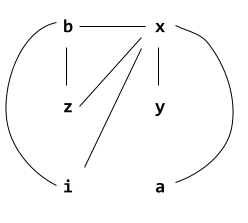
\includegraphics[scale=0.6]{../assets/loc_use1.png}
\end{center}
This is a graph where if there are two variables that had to be live at the same time, then there is an edge. How do we make it so we can have a set of locations where each variable can be assigned to a register that's different from all the things it conflicts with? This is known as \textbf{graph coloring}.

\end{document}